\documentclass[twoside]{book}

% Packages required by doxygen
\usepackage{calc}
\usepackage{doxygen}
\usepackage{graphicx}
\usepackage[utf8]{inputenc}
\usepackage{makeidx}
\usepackage{multicol}
\usepackage{multirow}
\usepackage{textcomp}
\usepackage[table]{xcolor}

% Font selection
\usepackage[T1]{fontenc}
\usepackage{mathptmx}
\usepackage[scaled=.90]{helvet}
\usepackage{courier}
\usepackage{amssymb}
\usepackage{sectsty}
\renewcommand{\familydefault}{\sfdefault}
\allsectionsfont{%
  \fontseries{bc}\selectfont%
  \color{darkgray}%
}
\renewcommand{\DoxyLabelFont}{%
  \fontseries{bc}\selectfont%
  \color{darkgray}%
}

% Page & text layout
\usepackage{geometry}
\geometry{%
  a4paper,%
  top=2.5cm,%
  bottom=2.5cm,%
  left=2.5cm,%
  right=2.5cm%
}
\tolerance=750
\hfuzz=15pt
\hbadness=750
\setlength{\emergencystretch}{15pt}
\setlength{\parindent}{0cm}
\setlength{\parskip}{0.2cm}
\makeatletter
\renewcommand{\paragraph}{%
  \@startsection{paragraph}{4}{0ex}{-1.0ex}{1.0ex}{%
    \normalfont\normalsize\bfseries\SS@parafont%
  }%
}
\renewcommand{\subparagraph}{%
  \@startsection{subparagraph}{5}{0ex}{-1.0ex}{1.0ex}{%
    \normalfont\normalsize\bfseries\SS@subparafont%
  }%
}
\makeatother

% Headers & footers
\usepackage{fancyhdr}
\pagestyle{fancyplain}
\fancyhead[LE]{\fancyplain{}{\bfseries\thepage}}
\fancyhead[CE]{\fancyplain{}{}}
\fancyhead[RE]{\fancyplain{}{\bfseries\leftmark}}
\fancyhead[LO]{\fancyplain{}{\bfseries\rightmark}}
\fancyhead[CO]{\fancyplain{}{}}
\fancyhead[RO]{\fancyplain{}{\bfseries\thepage}}
\fancyfoot[LE]{\fancyplain{}{}}
\fancyfoot[CE]{\fancyplain{}{}}
\fancyfoot[RE]{\fancyplain{}{\bfseries\scriptsize Generated on Sun Jul 13 2014 01\-:42\-:53 for Kinao by Doxygen }}
\fancyfoot[LO]{\fancyplain{}{\bfseries\scriptsize Generated on Sun Jul 13 2014 01\-:42\-:53 for Kinao by Doxygen }}
\fancyfoot[CO]{\fancyplain{}{}}
\fancyfoot[RO]{\fancyplain{}{}}
\renewcommand{\footrulewidth}{0.4pt}
\renewcommand{\chaptermark}[1]{%
  \markboth{#1}{}%
}
\renewcommand{\sectionmark}[1]{%
  \markright{\thesection\ #1}%
}

% Indices & bibliography
\usepackage{natbib}
\usepackage[titles]{tocloft}
\setcounter{tocdepth}{3}
\setcounter{secnumdepth}{5}
\makeindex

% Hyperlinks (required, but should be loaded last)
\usepackage{ifpdf}
\ifpdf
  \usepackage[pdftex,pagebackref=true]{hyperref}
\else
  \usepackage[ps2pdf,pagebackref=true]{hyperref}
\fi
\hypersetup{%
  colorlinks=true,%
  linkcolor=blue,%
  citecolor=blue,%
  unicode%
}

% Custom commands
\newcommand{\clearemptydoublepage}{%
  \newpage{\pagestyle{empty}\cleardoublepage}%
}


%===== C O N T E N T S =====

\begin{document}

% Titlepage & ToC
\hypersetup{pageanchor=false}
\pagenumbering{roman}
\begin{titlepage}
\vspace*{7cm}
\begin{center}%
{\Large Kinao }\\
\vspace*{1cm}
{\large Generated by Doxygen 1.8.6}\\
\vspace*{0.5cm}
{\small Sun Jul 13 2014 01:42:53}\\
\end{center}
\end{titlepage}
\clearemptydoublepage
\tableofcontents
\clearemptydoublepage
\pagenumbering{arabic}
\hypersetup{pageanchor=true}

%--- Begin generated contents ---
\chapter{Hierarchical Index}
\section{Class Hierarchy}
This inheritance list is sorted roughly, but not completely, alphabetically\-:\begin{DoxyCompactList}
\item \contentsline{section}{Joint}{\pageref{class_joint}}{}
\begin{DoxyCompactList}
\item \contentsline{section}{Head}{\pageref{class_head}}{}
\item \contentsline{section}{L\-Arm}{\pageref{class_l_arm}}{}
\item \contentsline{section}{L\-Leg}{\pageref{class_l_leg}}{}
\item \contentsline{section}{R\-Arm}{\pageref{class_r_arm}}{}
\item \contentsline{section}{R\-Leg}{\pageref{class_r_leg}}{}
\end{DoxyCompactList}
\item \contentsline{section}{Xn\-Reference\-Axis}{\pageref{struct_xn_reference_axis}}{}
\end{DoxyCompactList}

\chapter{Class Index}
\section{\-Class \-List}
\-Here are the classes, structs, unions and interfaces with brief descriptions\-:\begin{DoxyCompactList}
\item\contentsline{section}{\hyperlink{class_head}{\-Head} \\*\-Aqui se describe la clase derivada \char`\"{}\-Head\char`\"{} }{\pageref{class_head}}{}
\item\contentsline{section}{\hyperlink{class_joint}{\-Joint} \\*\-Aqui se describe la clase base \char`\"{}\-Joint\char`\"{} }{\pageref{class_joint}}{}
\item\contentsline{section}{\hyperlink{class_l_arm}{\-L\-Arm} \\*\-Esta es la clase que describe el comportamiento para los brazos }{\pageref{class_l_arm}}{}
\item\contentsline{section}{\hyperlink{class_l_leg}{\-L\-Leg} }{\pageref{class_l_leg}}{}
\item\contentsline{section}{\hyperlink{class_r_arm}{\-R\-Arm} }{\pageref{class_r_arm}}{}
\item\contentsline{section}{\hyperlink{class_r_leg}{\-R\-Leg} }{\pageref{class_r_leg}}{}
\item\contentsline{section}{\hyperlink{struct_xn_reference_axis}{\-Xn\-Reference\-Axis} }{\pageref{struct_xn_reference_axis}}{}
\end{DoxyCompactList}

\chapter{Class Documentation}
\hypertarget{class_head}{\section{Head Class Reference}
\label{class_head}\index{Head@{Head}}
}


Aqui se describe la clase derivada \char`\"{}\-Head\char`\"{}.  




{\ttfamily \#include $<$joint.\-h$>$}

Inheritance diagram for Head\-:\begin{figure}[H]
\begin{center}
\leavevmode
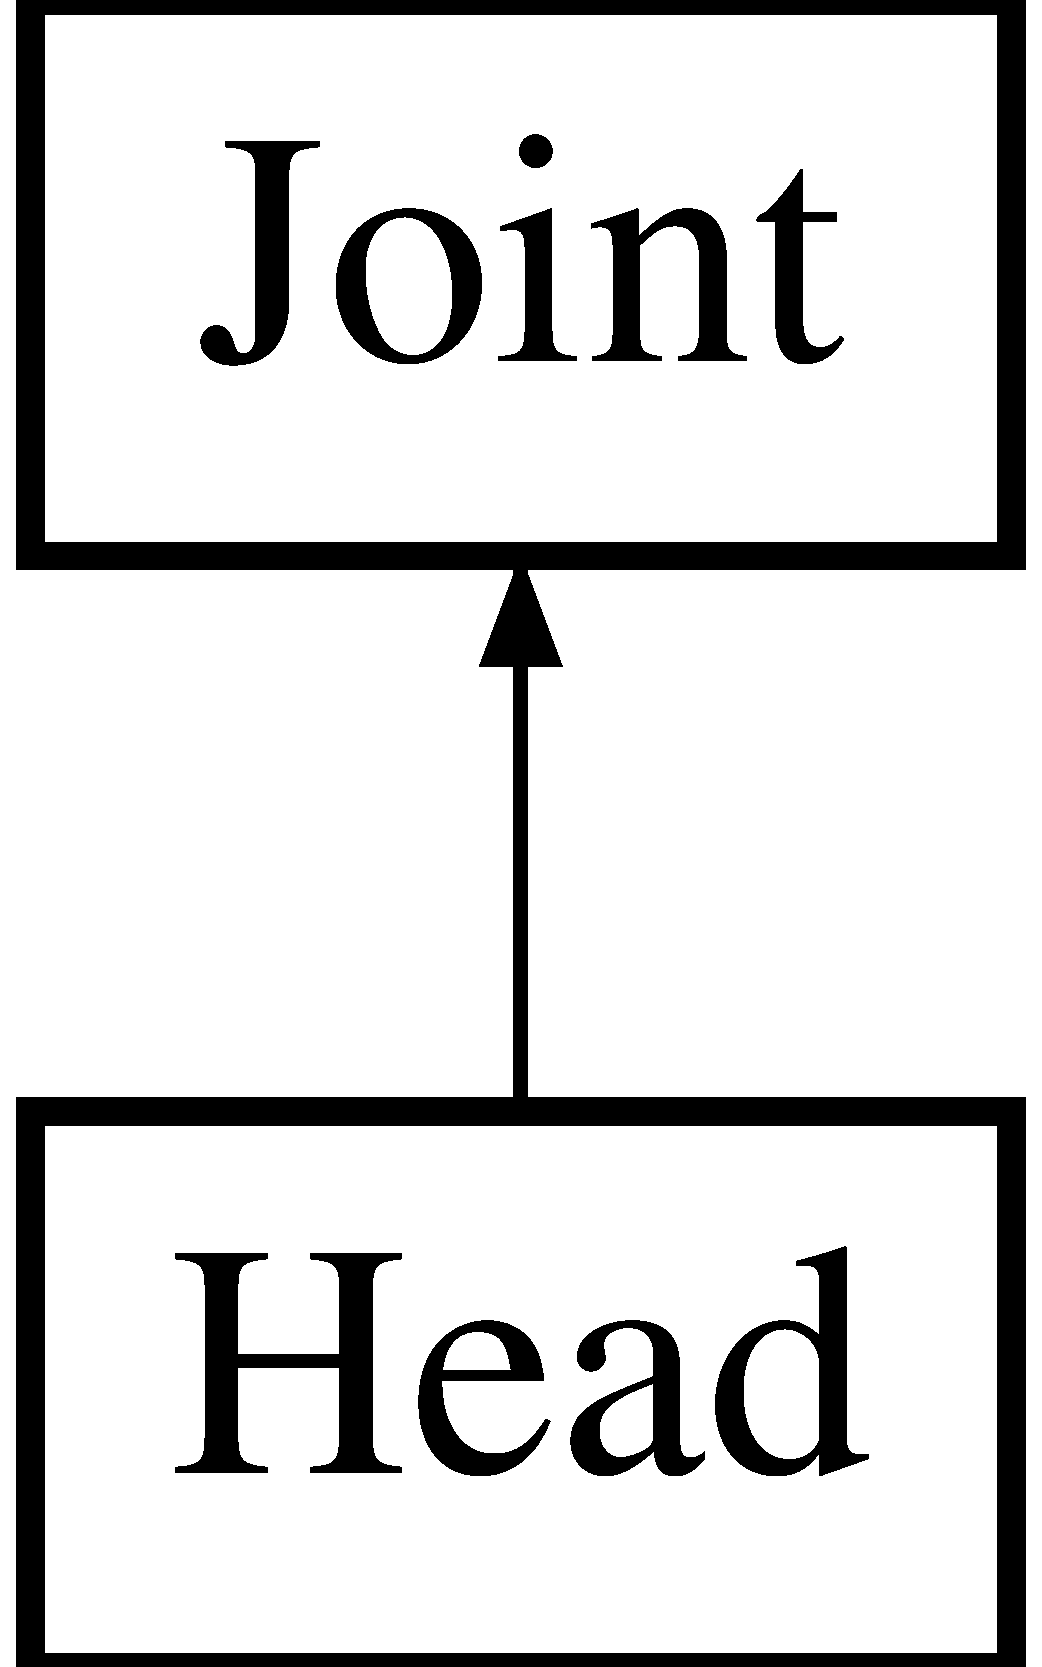
\includegraphics[height=2.000000cm]{class_head}
\end{center}
\end{figure}
\subsection*{Public Member Functions}
\begin{DoxyCompactItemize}
\item 
\hypertarget{class_head_a0a4e931e188a25b60f6b992ff32f7bfa}{\hyperlink{class_head_a0a4e931e188a25b60f6b992ff32f7bfa}{Head} ()}\label{class_head_a0a4e931e188a25b60f6b992ff32f7bfa}

\begin{DoxyCompactList}\small\item\em Declaracion de la clase derivada \char`\"{}\-Head\char`\"{} y su funcionalidad. \end{DoxyCompactList}\item 
\hypertarget{class_head_a502987ba6c8d6b615977150dd565fc27}{virtual \hyperlink{class_head_a502987ba6c8d6b615977150dd565fc27}{$\sim$\-Head} (void)}\label{class_head_a502987ba6c8d6b615977150dd565fc27}

\begin{DoxyCompactList}\small\item\em Constructor del Objeto. \end{DoxyCompactList}\item 
virtual float \hyperlink{class_head_ad57a93c84de0a6681dce1dbcdc87823c}{get\-Head\-Pitch} (Xn\-User\-I\-D, xn\-::\-User\-Generator)
\begin{DoxyCompactList}\small\item\em Obtiene el angulo que se determina a partir del kinect. \end{DoxyCompactList}\item 
\hypertarget{class_head_a6f624a1b326a840aad5221608809f40f}{virtual float \hyperlink{class_head_a6f624a1b326a840aad5221608809f40f}{set\-Head\-Pitch} (float, float \&, float \&)}\label{class_head_a6f624a1b326a840aad5221608809f40f}

\begin{DoxyCompactList}\small\item\em Genera el angulo necesario para mover el N\-A\-O. \end{DoxyCompactList}\end{DoxyCompactItemize}


\subsection{Detailed Description}
Aqui se describe la clase derivada \char`\"{}\-Head\char`\"{}. 

\subsection{Member Function Documentation}
\hypertarget{class_head_ad57a93c84de0a6681dce1dbcdc87823c}{\index{Head@{Head}!get\-Head\-Pitch@{get\-Head\-Pitch}}
\index{get\-Head\-Pitch@{get\-Head\-Pitch}!Head@{Head}}
\subsubsection[{get\-Head\-Pitch}]{\setlength{\rightskip}{0pt plus 5cm}float Head\-::get\-Head\-Pitch (
\begin{DoxyParamCaption}
\item[{Xn\-User\-I\-D}]{user, }
\item[{xn\-::\-User\-Generator}]{guser}
\end{DoxyParamCaption}
)\hspace{0.3cm}{\ttfamily [virtual]}}}\label{class_head_ad57a93c84de0a6681dce1dbcdc87823c}


Obtiene el angulo que se determina a partir del kinect. 

Obtiene el angulo real dado por el kinect del movimiento frontal de la cabeza.

Destructor del Objeto 

The documentation for this class was generated from the following files\-:\begin{DoxyCompactItemize}
\item 
/home/daniel/\-U\-C\-R/\-Ey\-A\-Team/kinect/\-Open\-N\-I\-\_\-\-N\-I\-T\-E\-\_\-\-Installer-\/\-Linux64-\/0.\-27/\-Open\-N\-I-\/\-Bin-\/\-Dev-\/\-Linux-\/x64-\/v1.\-5.\-4.\-0/\-Samples/\-Ni\-Simple\-Skeleton/kinao/joint.\-h\item 
/home/daniel/\-U\-C\-R/\-Ey\-A\-Team/kinect/\-Open\-N\-I\-\_\-\-N\-I\-T\-E\-\_\-\-Installer-\/\-Linux64-\/0.\-27/\-Open\-N\-I-\/\-Bin-\/\-Dev-\/\-Linux-\/x64-\/v1.\-5.\-4.\-0/\-Samples/\-Ni\-Simple\-Skeleton/kinao/head.\-cpp\end{DoxyCompactItemize}

\hypertarget{class_joint}{\section{Joint Class Reference}
\label{class_joint}\index{Joint@{Joint}}
}


Aqui se describe la clase base \char`\"{}\-Joint\char`\"{}.  




{\ttfamily \#include $<$joint.\-h$>$}

Inheritance diagram for Joint\-:\begin{figure}[H]
\begin{center}
\leavevmode
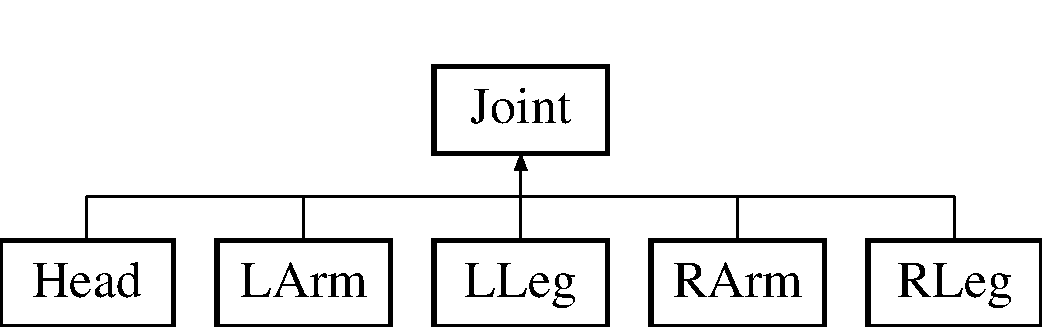
\includegraphics[height=2.000000cm]{class_joint}
\end{center}
\end{figure}
\subsection*{Public Member Functions}
\begin{DoxyCompactItemize}
\item 
\hypertarget{class_joint_a79a7a4715b2166714e039d7c7c5ea3b4}{\hyperlink{class_joint_a79a7a4715b2166714e039d7c7c5ea3b4}{Joint} ()}\label{class_joint_a79a7a4715b2166714e039d7c7c5ea3b4}

\begin{DoxyCompactList}\small\item\em Esta es la decralarion de la funcionalidad de la clase base \char`\"{}\-Joint\char`\"{}, de aqui se deriban las demas. \end{DoxyCompactList}\item 
\hypertarget{class_joint_ac9749eeeac49e9861554f2d580cc020d}{virtual \hyperlink{class_joint_ac9749eeeac49e9861554f2d580cc020d}{$\sim$\-Joint} (void)}\label{class_joint_ac9749eeeac49e9861554f2d580cc020d}

\begin{DoxyCompactList}\small\item\em Constructor del Objeto. \end{DoxyCompactList}\item 
virtual float \hyperlink{class_joint_a1b4c78e285a1d96bbde889d4979828fa}{length} (float\mbox{[}3\mbox{]}, float\mbox{[}3\mbox{]})
\begin{DoxyCompactList}\small\item\em Destructor del Objeto. \end{DoxyCompactList}\item 
virtual float \hyperlink{class_joint_ab4a853045a69e77e8b67d195be145eed}{angle} (float, float, float)
\item 
virtual float \hyperlink{class_joint_a52f2f6003f4cff059847d959488622a1}{get\-Angle} (Xn\-Vector3\-D, Xn\-Vector3\-D, Xn\-Vector3\-D)
\begin{DoxyCompactList}\small\item\em L1,L2,L3(\-L3 es el opuesto del angulo a determinar) \end{DoxyCompactList}\item 
virtual Xn\-Vector3\-D \hyperlink{class_joint_ac59f570adbaf039bbe0f4173e5e7e2ce}{get\-Normal\-Vector} (Xn\-Vector3\-D, Xn\-Vector3\-D, Xn\-Vector3\-D)
\begin{DoxyCompactList}\small\item\em Genera el vector resultante de realizar el producto cruz entre los 2 vectores coplanares. \end{DoxyCompactList}\item 
virtual Xn\-Vector3\-D \hyperlink{class_joint_af5590ba3d5bfc4e27a43036a1d394629}{get\-Proyection\-Vector} (Xn\-Vector3\-D, Xn\-Vector3\-D)
\begin{DoxyCompactList}\small\item\em Obtiene el vector resultante de proyectar un vector sobre otro. \end{DoxyCompactList}\item 
virtual Xn\-Float \hyperlink{class_joint_a06ed69732a17f61fa6ce9fa5ba2541ea}{get\-Proyection} (Xn\-Vector3\-D Vector1, Xn\-Vector3\-D Vector2)
\begin{DoxyCompactList}\small\item\em Obtiene la constante de la proyeccion. \end{DoxyCompactList}\item 
virtual \hyperlink{struct_xn_reference_axis}{Xn\-Reference\-Axis} \hyperlink{class_joint_a603eab4701f005bc6a39911897eb6c7d}{generate\-Reference} (Xn\-Vector3\-D, Xn\-Vector3\-D, Xn\-Vector3\-D)
\begin{DoxyCompactList}\small\item\em Construye un nuevo eje de coordenadas a partir de 3 vectores otrtogonales. \end{DoxyCompactList}\end{DoxyCompactItemize}


\subsection{Detailed Description}
Aqui se describe la clase base \char`\"{}\-Joint\char`\"{}. 

\subsection{Member Function Documentation}
\hypertarget{class_joint_ab4a853045a69e77e8b67d195be145eed}{\index{Joint@{Joint}!angle@{angle}}
\index{angle@{angle}!Joint@{Joint}}
\subsubsection[{angle}]{\setlength{\rightskip}{0pt plus 5cm}float Joint\-::angle (
\begin{DoxyParamCaption}
\item[{float}]{R\-L1, }
\item[{float}]{R\-L2, }
\item[{float}]{I\-M\-L3}
\end{DoxyParamCaption}
)\hspace{0.3cm}{\ttfamily [virtual]}}}\label{class_joint_ab4a853045a69e77e8b67d195be145eed}
P1\mbox{[}3\mbox{]},P2\mbox{[}3\mbox{]} Determina el angulo entre 3 puntos dadas las 3 lineas descritas por estos puntos El angulo a determinar viene dado por la linea imaginaria que esta opuesta a este angulo I\-M\-L3 es el segmento contrario al angulo por determinar, el cual no existe, es I\-Maginario \hypertarget{class_joint_a603eab4701f005bc6a39911897eb6c7d}{\index{Joint@{Joint}!generate\-Reference@{generate\-Reference}}
\index{generate\-Reference@{generate\-Reference}!Joint@{Joint}}
\subsubsection[{generate\-Reference}]{\setlength{\rightskip}{0pt plus 5cm}{\bf Xn\-Reference\-Axis} Joint\-::generate\-Reference (
\begin{DoxyParamCaption}
\item[{Xn\-Vector3\-D}]{J1, }
\item[{Xn\-Vector3\-D}]{J2, }
\item[{Xn\-Vector3\-D}]{J3}
\end{DoxyParamCaption}
)\hspace{0.3cm}{\ttfamily [virtual]}}}\label{class_joint_a603eab4701f005bc6a39911897eb6c7d}


Construye un nuevo eje de coordenadas a partir de 3 vectores otrtogonales. 

Este método genera un nuevo eje de referencia centrado en un \hyperlink{class_joint}{Joint}. Point\-Normal1 es un nuevo \hyperlink{class_joint}{Joint} para calcular una de las normales que será parte del marco de referencia

Utilizamos el struct \hyperlink{struct_xn_reference_axis}{Xn\-Reference\-Axis} definido previamente para almacenar el nuevo marco de referencia \hypertarget{class_joint_a52f2f6003f4cff059847d959488622a1}{\index{Joint@{Joint}!get\-Angle@{get\-Angle}}
\index{get\-Angle@{get\-Angle}!Joint@{Joint}}
\subsubsection[{get\-Angle}]{\setlength{\rightskip}{0pt plus 5cm}float Joint\-::get\-Angle (
\begin{DoxyParamCaption}
\item[{Xn\-Vector3\-D}]{J1, }
\item[{Xn\-Vector3\-D}]{J2, }
\item[{Xn\-Vector3\-D}]{J3}
\end{DoxyParamCaption}
)\hspace{0.3cm}{\ttfamily [virtual]}}}\label{class_joint_a52f2f6003f4cff059847d959488622a1}


L1,L2,L3(\-L3 es el opuesto del angulo a determinar) 

J2 es la articulacion a la que se va a sacar el angulo.

Aunque se podria, no se crea una funcion get\-Angle aqui porque se necesitan pasar los parametros que usa el kinect para cada una de las posiciones, lo que se quiere es simplemente decir head.\-get\-Angle y que se obtenga el de la cabeza. Se pordria hacer, pero inicializando todos los joints y que se esten actualizando en tiempo real en la clasd \hyperlink{class_joint}{Joint}, para luego simplemente llamarlos desde las respectivas subclases igualando el valor actual del \hyperlink{class_joint}{Joint} en x,y,z a mi variable dentro de la subclase, luego como el objeto es de tipo \hyperlink{class_head}{Head}, entonces el automaticamente sabe que las variables que debe pasar son las corerspondientes a los puntos que describen el angulo del cuello. Por ahora queda como mejora Determina directamente el angulo que hay en el segundo vector Se toman los tres vectores y se determina la distancia entre ellos, donde Imag3 es la distancia opuesta el J2 \hypertarget{class_joint_ac59f570adbaf039bbe0f4173e5e7e2ce}{\index{Joint@{Joint}!get\-Normal\-Vector@{get\-Normal\-Vector}}
\index{get\-Normal\-Vector@{get\-Normal\-Vector}!Joint@{Joint}}
\subsubsection[{get\-Normal\-Vector}]{\setlength{\rightskip}{0pt plus 5cm}Xn\-Vector3\-D Joint\-::get\-Normal\-Vector (
\begin{DoxyParamCaption}
\item[{Xn\-Vector3\-D}]{J1, }
\item[{Xn\-Vector3\-D}]{J2, }
\item[{Xn\-Vector3\-D}]{J3}
\end{DoxyParamCaption}
)\hspace{0.3cm}{\ttfamily [virtual]}}}\label{class_joint_ac59f570adbaf039bbe0f4173e5e7e2ce}


Genera el vector resultante de realizar el producto cruz entre los 2 vectores coplanares. 

J2 es el punto de unión de los vectores J2-\/$>$J1 y J2-\/$>$J3, a los cuales se les sacará el vector normal. Generamos 2 vectores a partir de los cuales calcularemos el producto cruz, Vector1 X Vector2 = Vector\-Normal

Para Vector1 = J2-\/$>$J1

Para Vector2 = J2-\/$>$J3

Generamos el vector ortogonal Vector\-Normal \hypertarget{class_joint_a06ed69732a17f61fa6ce9fa5ba2541ea}{\index{Joint@{Joint}!get\-Proyection@{get\-Proyection}}
\index{get\-Proyection@{get\-Proyection}!Joint@{Joint}}
\subsubsection[{get\-Proyection}]{\setlength{\rightskip}{0pt plus 5cm}Xn\-Float Joint\-::get\-Proyection (
\begin{DoxyParamCaption}
\item[{Xn\-Vector3\-D}]{Vector1, }
\item[{Xn\-Vector3\-D}]{Vector2}
\end{DoxyParamCaption}
)\hspace{0.3cm}{\ttfamily [virtual]}}}\label{class_joint_a06ed69732a17f61fa6ce9fa5ba2541ea}


Obtiene la constante de la proyeccion. 

Calculamos la proyección del Vector1 sobre el Vector2. Generamos el vector en el cual se va a guardar la proyección resultante

Calculamos el producto punto entre Vector1 y Vector2

Calculamos la norma del Vector2

Ahora calculamos la constante que multiplica al vector sobre el cual estamos proyectando para generar el nuevo vector proyección \hypertarget{class_joint_af5590ba3d5bfc4e27a43036a1d394629}{\index{Joint@{Joint}!get\-Proyection\-Vector@{get\-Proyection\-Vector}}
\index{get\-Proyection\-Vector@{get\-Proyection\-Vector}!Joint@{Joint}}
\subsubsection[{get\-Proyection\-Vector}]{\setlength{\rightskip}{0pt plus 5cm}Xn\-Vector3\-D Joint\-::get\-Proyection\-Vector (
\begin{DoxyParamCaption}
\item[{Xn\-Vector3\-D}]{Vector1, }
\item[{Xn\-Vector3\-D}]{Vector2}
\end{DoxyParamCaption}
)\hspace{0.3cm}{\ttfamily [virtual]}}}\label{class_joint_af5590ba3d5bfc4e27a43036a1d394629}


Obtiene el vector resultante de proyectar un vector sobre otro. 

Calculamos la proyección del Vector1 sobre el Vector2. Generamos el vector en el cual se va a guardar la proyección resultante

Calculamos el producto punto entre Vector1 y Vector2

Calculamos la norma del Vector2 \hypertarget{class_joint_a1b4c78e285a1d96bbde889d4979828fa}{\index{Joint@{Joint}!length@{length}}
\index{length@{length}!Joint@{Joint}}
\subsubsection[{length}]{\setlength{\rightskip}{0pt plus 5cm}float Joint\-::length (
\begin{DoxyParamCaption}
\item[{float}]{p1\mbox{[}3\mbox{]}, }
\item[{float}]{p2\mbox{[}3\mbox{]}}
\end{DoxyParamCaption}
)\hspace{0.3cm}{\ttfamily [virtual]}}}\label{class_joint_a1b4c78e285a1d96bbde889d4979828fa}


Destructor del Objeto. 

Determina el vector que va de P1 a P2 Determina el vector que va de P1 a P2 

The documentation for this class was generated from the following files\-:\begin{DoxyCompactItemize}
\item 
/home/daniel/\-U\-C\-R/\-Ey\-A\-Team/kinect/\-Open\-N\-I\-\_\-\-N\-I\-T\-E\-\_\-\-Installer-\/\-Linux64-\/0.\-27/\-Open\-N\-I-\/\-Bin-\/\-Dev-\/\-Linux-\/x64-\/v1.\-5.\-4.\-0/\-Samples/\-Ni\-Simple\-Skeleton/kinao/joint.\-h\item 
/home/daniel/\-U\-C\-R/\-Ey\-A\-Team/kinect/\-Open\-N\-I\-\_\-\-N\-I\-T\-E\-\_\-\-Installer-\/\-Linux64-\/0.\-27/\-Open\-N\-I-\/\-Bin-\/\-Dev-\/\-Linux-\/x64-\/v1.\-5.\-4.\-0/\-Samples/\-Ni\-Simple\-Skeleton/kinao/joint.\-cpp\item 
/home/daniel/\-U\-C\-R/\-Ey\-A\-Team/kinect/\-Open\-N\-I\-\_\-\-N\-I\-T\-E\-\_\-\-Installer-\/\-Linux64-\/0.\-27/\-Open\-N\-I-\/\-Bin-\/\-Dev-\/\-Linux-\/x64-\/v1.\-5.\-4.\-0/\-Samples/\-Ni\-Simple\-Skeleton/kinao/normal.\-cpp\end{DoxyCompactItemize}

\hypertarget{class_l_arm}{\section{\-Referencia de \-Clase \-L\-Arm}
\label{class_l_arm}\index{\-L\-Arm@{\-L\-Arm}}
}


\-Esta es la clase que describe el comportamiento para el brazo izquierdo.  




{\ttfamily \#include $<$joint.\-h$>$}

\-Diagrama de herencia para \-L\-Arm\-:\begin{figure}[H]
\begin{center}
\leavevmode
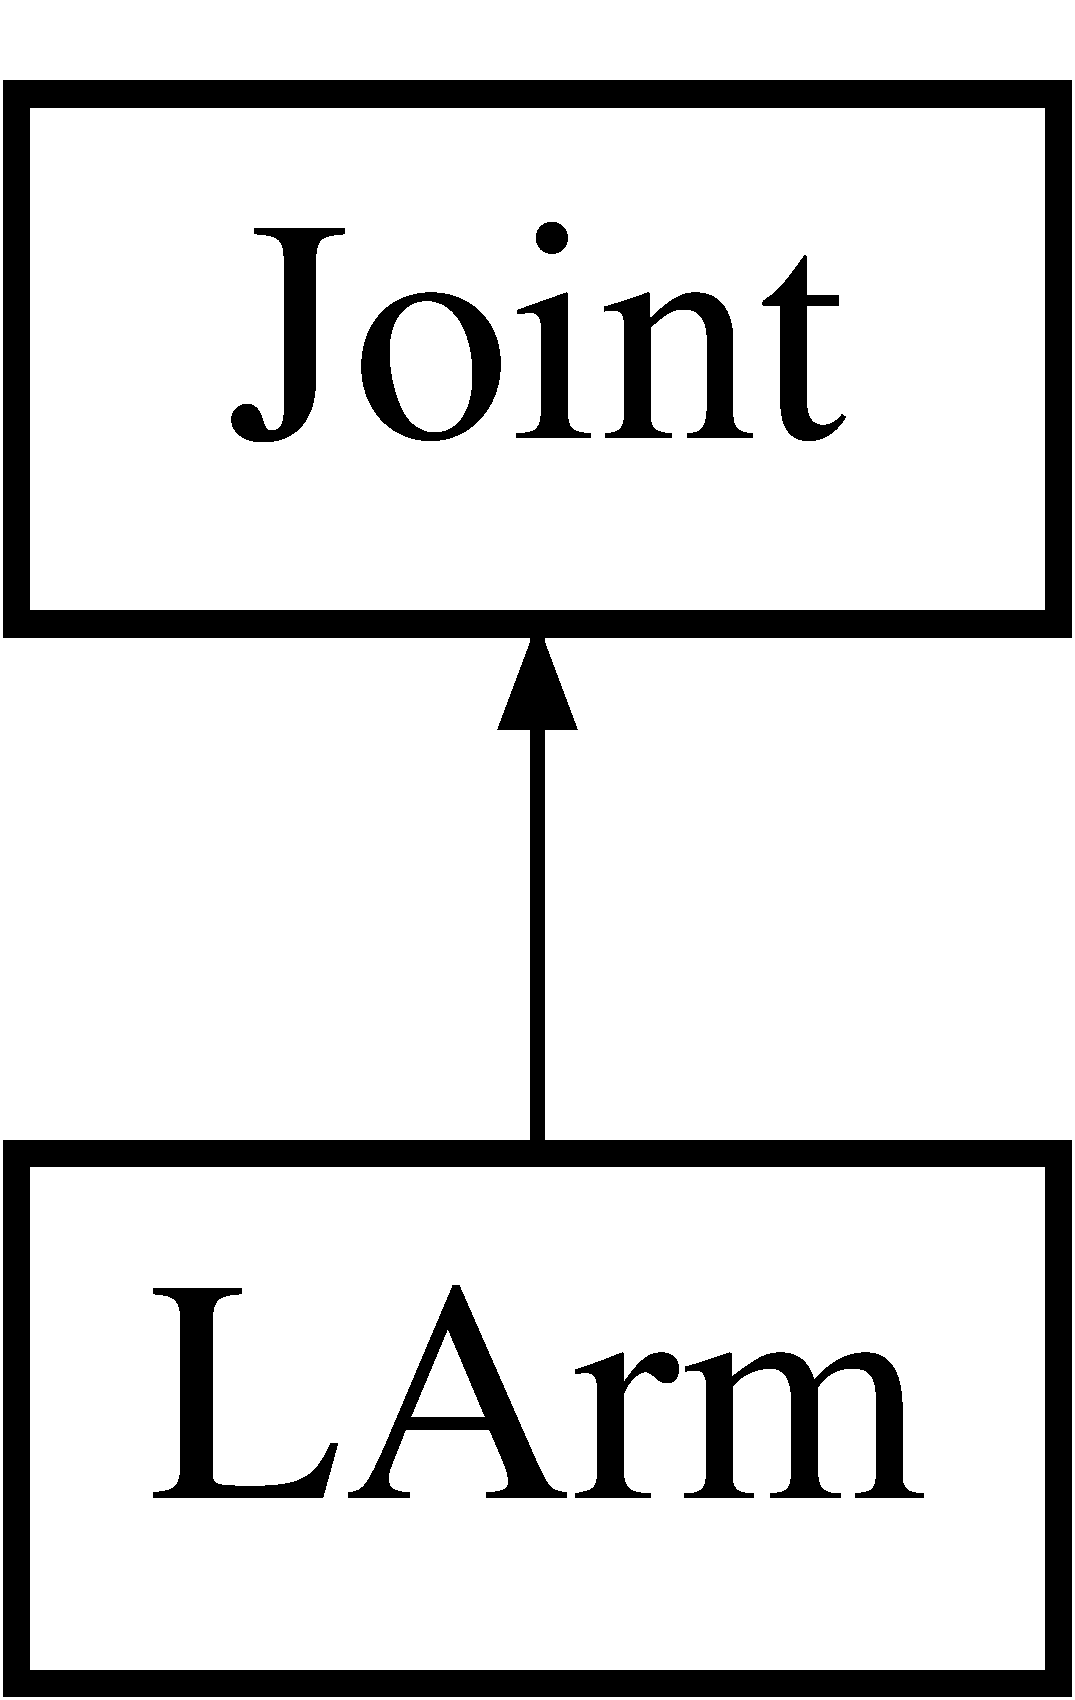
\includegraphics[height=2.000000cm]{class_l_arm}
\end{center}
\end{figure}
\subsection*{\-Funciones \-Miembro \-Públicas}
\begin{itemize}
\item 
virtual float \hyperlink{class_l_arm_aca3aa8c68dedd1c7fb1e0ed9ba55b239}{get\-Elbow\-Roll} (\-Xn\-User\-I\-D, xn\-::\-User\-Generator)
\begin{itemize}\small\item\em \-Obtiene el ángulo que se determina a partir del kinect del codo. \end{itemize}\item 
\hypertarget{class_l_arm_a19580475d6f1d5ae421a419a090f835e}{virtual float \hyperlink{class_l_arm_a19580475d6f1d5ae421a419a090f835e}{set\-Elbow\-Roll} (float, float \&, float \&)}\label{class_l_arm_a19580475d6f1d5ae421a419a090f835e}

\begin{itemize}\small\item\em \-Genera el ángulo al que se necesita mover el \-N\-A\-O. \end{itemize}\item 
\hypertarget{class_l_arm_a25b46c7a95c135f5020800b78a28d24a}{virtual float \hyperlink{class_l_arm_a25b46c7a95c135f5020800b78a28d24a}{get\-Shoulder\-Roll} (\-Xn\-User\-I\-D, xn\-::\-User\-Generator)}\label{class_l_arm_a25b46c7a95c135f5020800b78a28d24a}

\begin{itemize}\small\item\em \-Obtiene el ángulo que se determina a partir del kinect del hombro. \end{itemize}\item 
\hypertarget{class_l_arm_ada7589a6dabadd906736f76e9d71d9c5}{virtual float \hyperlink{class_l_arm_ada7589a6dabadd906736f76e9d71d9c5}{set\-Shoulder\-Roll} (float, float \&, float \&)}\label{class_l_arm_ada7589a6dabadd906736f76e9d71d9c5}

\begin{itemize}\small\item\em \-Genera el ángulo al que es necesario mover el \-N\-A\-O. \end{itemize}\item 
virtual float \hyperlink{class_l_arm_a45c25b7614431e4a3e39bfcf977a3de7}{get\-Elbow\-Yaw} (\-Xn\-User\-I\-D, xn\-::\-User\-Generator)
\item 
\hypertarget{class_l_arm_a536c8e6957dfc9e2b8a9d3c0ee3b8f52}{virtual float \hyperlink{class_l_arm_a536c8e6957dfc9e2b8a9d3c0ee3b8f52}{set\-Elbow\-Yaw} (float, float \&, float \&)}\label{class_l_arm_a536c8e6957dfc9e2b8a9d3c0ee3b8f52}

\end{itemize}


\subsection{\-Descripción \-Detallada}
\-Esta es la clase que describe el comportamiento para el brazo izquierdo. 

\subsection{\-Documentación de \-Función \-Miembro}
\hypertarget{class_l_arm_aca3aa8c68dedd1c7fb1e0ed9ba55b239}{\index{\-L\-Arm@{\-L\-Arm}!get\-Elbow\-Roll@{get\-Elbow\-Roll}}
\index{get\-Elbow\-Roll@{get\-Elbow\-Roll}!LArm@{\-L\-Arm}}
\subsubsection[{get\-Elbow\-Roll}]{\setlength{\rightskip}{0pt plus 5cm}float {\bf \-L\-Arm\-::get\-Elbow\-Roll} (
[{\-Xn\-User\-I\-D}]{user, }
[{xn\-::\-User\-Generator}]{guser}
)\hspace{0.3cm}{\ttfamily  \mbox{[}virtual\mbox{]}}}}\label{class_l_arm_aca3aa8c68dedd1c7fb1e0ed9ba55b239}


\-Primero se obtienen los puntos que van a determinar el ángulo de codo, se toman los puntos de la muñeca, codo y hombro.\\
\-Luego, utilizando las funciones descritas en la función base Joint, se procede a determinar el ángulo para el movimiento del codo. 


 \hypertarget{class_l_arm_a45c25b7614431e4a3e39bfcf977a3de7}{\index{\-L\-Arm@{\-L\-Arm}!get\-Elbow\-Yaw@{get\-Elbow\-Yaw}}
\index{get\-Elbow\-Yaw@{get\-Elbow\-Yaw}!LArm@{\-L\-Arm}}
\subsubsection[{get\-Elbow\-Yaw}]{\setlength{\rightskip}{0pt plus 5cm}float {\bf \-L\-Arm\-::get\-Elbow\-Yaw} (
[{\-Xn\-User\-I\-D}]{user, }
[{xn\-::\-User\-Generator}]{guser}
)\hspace{0.3cm}{\ttfamily  \mbox{[}virtual\mbox{]}}}}\label{class_l_arm_a45c25b7614431e4a3e39bfcf977a3de7}
\-Marco de referencia en un momento anterior con punto central sobre el codo.

\-Se obtiene el vector el\-To\-Hand (codo -\/$>$ mano).

\-Se obtiene la proyección del vector el\-To\-Hand sobre el eje \-Z de la referencia en el codo.

\-Se obtiene el punto imaginario.

\-Se obtiene la proyección sobre el plano \-X\-Y, para ello obtenemos se forma entre la proyección y el vector el\-To\-Hand.

\-Se obtiene primer punto que es la proyección de la mano sobre el plano \-X\-Y.

\-Se obtiene el segundo punto sobre nuestro eje \-Y.

\-Se obtiene el ángulo entre la proyección entre el plano \-X\-Y y el eje \-Y.

\-Se determina el signo del ángulo para saber si rotamos el codo en sentido horario o antihorario \-Se obtiene la proyección del vector proy\-Vector\-Plane sobre el eje \-X de la referencia en el codo. 

\-La documentación para esta clase fue generada apartir de los archivos\-:\begin{itemize}
\item 
joint.\-h\item 
larm.\-cpp\end{itemize}

\hypertarget{class_l_leg}{\section{L\-Leg Class Reference}
\label{class_l_leg}\index{L\-Leg@{L\-Leg}}
}
Inheritance diagram for L\-Leg\-:\begin{figure}[H]
\begin{center}
\leavevmode
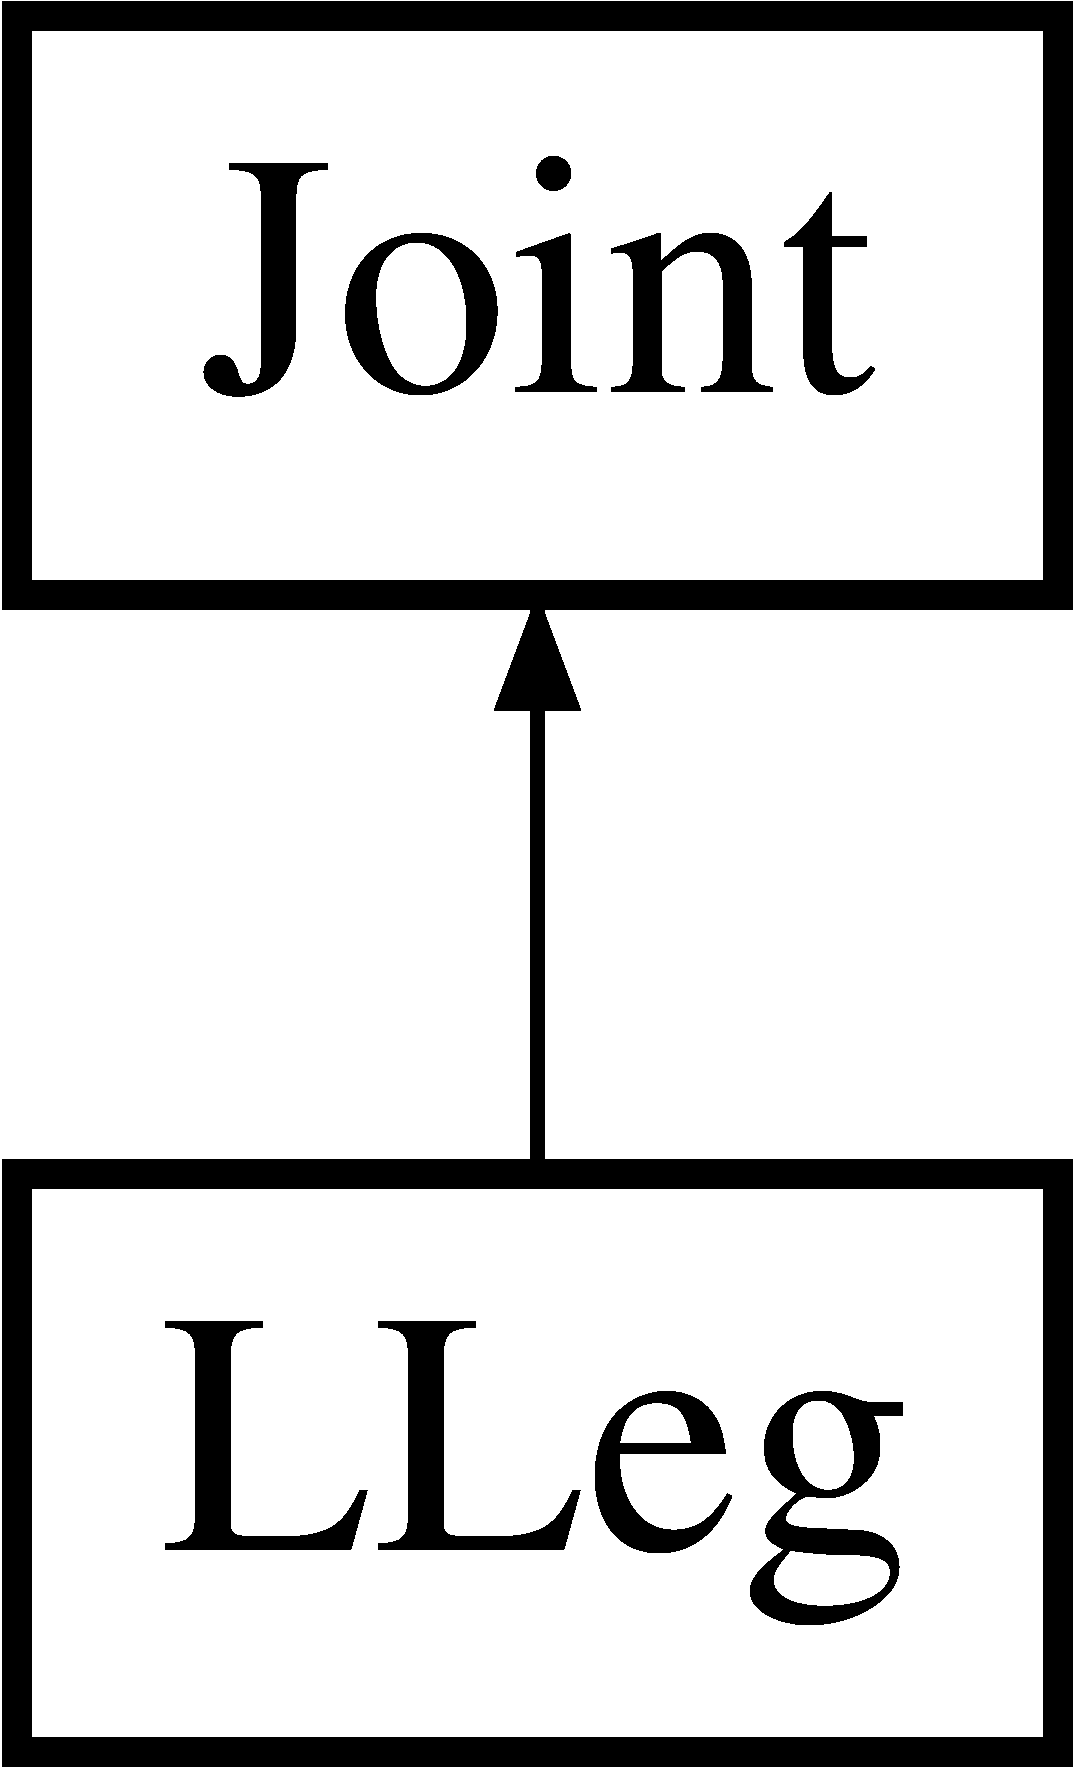
\includegraphics[height=2.000000cm]{class_l_leg}
\end{center}
\end{figure}
\subsection*{Public Member Functions}
\begin{DoxyCompactItemize}
\item 
virtual float \hyperlink{class_l_leg_ac0d2147e72701ad8202b758bb572735f}{get\-Hip\-Roll} (Xn\-User\-I\-D, xn\-::\-User\-Generator)
\begin{DoxyCompactList}\small\item\em Obtiene el angulo que se determina a partir del kinect del hombro. \end{DoxyCompactList}\item 
\hypertarget{class_l_leg_a200afc21f99236f2af57b95ea648573b}{virtual float \hyperlink{class_l_leg_a200afc21f99236f2af57b95ea648573b}{set\-Hip\-Roll} (float, float \&, float \&)}\label{class_l_leg_a200afc21f99236f2af57b95ea648573b}

\begin{DoxyCompactList}\small\item\em Genera el angulo necesario para mover el N\-A\-O. \end{DoxyCompactList}\item 
\hypertarget{class_l_leg_a4a31233e6def8edde81e5d694b7e0feb}{virtual float \hyperlink{class_l_leg_a4a31233e6def8edde81e5d694b7e0feb}{get\-Knee\-Pitch} (Xn\-User\-I\-D, xn\-::\-User\-Generator)}\label{class_l_leg_a4a31233e6def8edde81e5d694b7e0feb}

\begin{DoxyCompactList}\small\item\em Obtiene el angulo que se determina a partir del kinect. \end{DoxyCompactList}\item 
\hypertarget{class_l_leg_a15417e9792bbc9a2f398ed9127e3db11}{virtual float \hyperlink{class_l_leg_a15417e9792bbc9a2f398ed9127e3db11}{set\-Knee\-Pitch} (float, float \&, float \&)}\label{class_l_leg_a15417e9792bbc9a2f398ed9127e3db11}

\begin{DoxyCompactList}\small\item\em Genera el angulo necesario para mover el N\-A\-O. \end{DoxyCompactList}\item 
\hypertarget{class_l_leg_a85ec581c8db5d113a13be644a851753e}{virtual float \hyperlink{class_l_leg_a85ec581c8db5d113a13be644a851753e}{get\-Ankle\-Pitch} (Xn\-User\-I\-D, xn\-::\-User\-Generator)}\label{class_l_leg_a85ec581c8db5d113a13be644a851753e}

\begin{DoxyCompactList}\small\item\em Obtiene el angulo que se determina a partir del kinect. \end{DoxyCompactList}\item 
\hypertarget{class_l_leg_ab474375cb60e68fbf5790459b690b42f}{virtual float \hyperlink{class_l_leg_ab474375cb60e68fbf5790459b690b42f}{set\-Ankle\-Pitch} (float, float \&, float \&)}\label{class_l_leg_ab474375cb60e68fbf5790459b690b42f}

\begin{DoxyCompactList}\small\item\em Genera angulo para mover N\-A\-O. \end{DoxyCompactList}\end{DoxyCompactItemize}


\subsection{Member Function Documentation}
\hypertarget{class_l_leg_ac0d2147e72701ad8202b758bb572735f}{\index{L\-Leg@{L\-Leg}!get\-Hip\-Roll@{get\-Hip\-Roll}}
\index{get\-Hip\-Roll@{get\-Hip\-Roll}!LLeg@{L\-Leg}}
\subsubsection[{get\-Hip\-Roll}]{\setlength{\rightskip}{0pt plus 5cm}float L\-Leg\-::get\-Hip\-Roll (
\begin{DoxyParamCaption}
\item[{Xn\-User\-I\-D}]{user, }
\item[{xn\-::\-User\-Generator}]{guser}
\end{DoxyParamCaption}
)\hspace{0.3cm}{\ttfamily [virtual]}}}\label{class_l_leg_ac0d2147e72701ad8202b758bb572735f}


Obtiene el angulo que se determina a partir del kinect del hombro. 

Obtiene el angulo real dado por el kinect del movimiento del codo. 

The documentation for this class was generated from the following files\-:\begin{DoxyCompactItemize}
\item 
/home/daniel/\-U\-C\-R/\-Ey\-A\-Team/kinect/\-Open\-N\-I\-\_\-\-N\-I\-T\-E\-\_\-\-Installer-\/\-Linux64-\/0.\-27/\-Open\-N\-I-\/\-Bin-\/\-Dev-\/\-Linux-\/x64-\/v1.\-5.\-4.\-0/\-Samples/\-Ni\-Simple\-Skeleton/kinao/joint.\-h\item 
/home/daniel/\-U\-C\-R/\-Ey\-A\-Team/kinect/\-Open\-N\-I\-\_\-\-N\-I\-T\-E\-\_\-\-Installer-\/\-Linux64-\/0.\-27/\-Open\-N\-I-\/\-Bin-\/\-Dev-\/\-Linux-\/x64-\/v1.\-5.\-4.\-0/\-Samples/\-Ni\-Simple\-Skeleton/kinao/lleg.\-cpp\end{DoxyCompactItemize}

\hypertarget{class_r_arm}{\section{{\-R\-Arm \-Class \-Reference} \-R\-Arm}
\label{class_r_arm}\index{\-R\-Arm@{\-R\-Arm}}
}
\-Diagrama de herencia para \-R\-Arm\-:\begin{figure}[H]
\begin{center}
\leavevmode
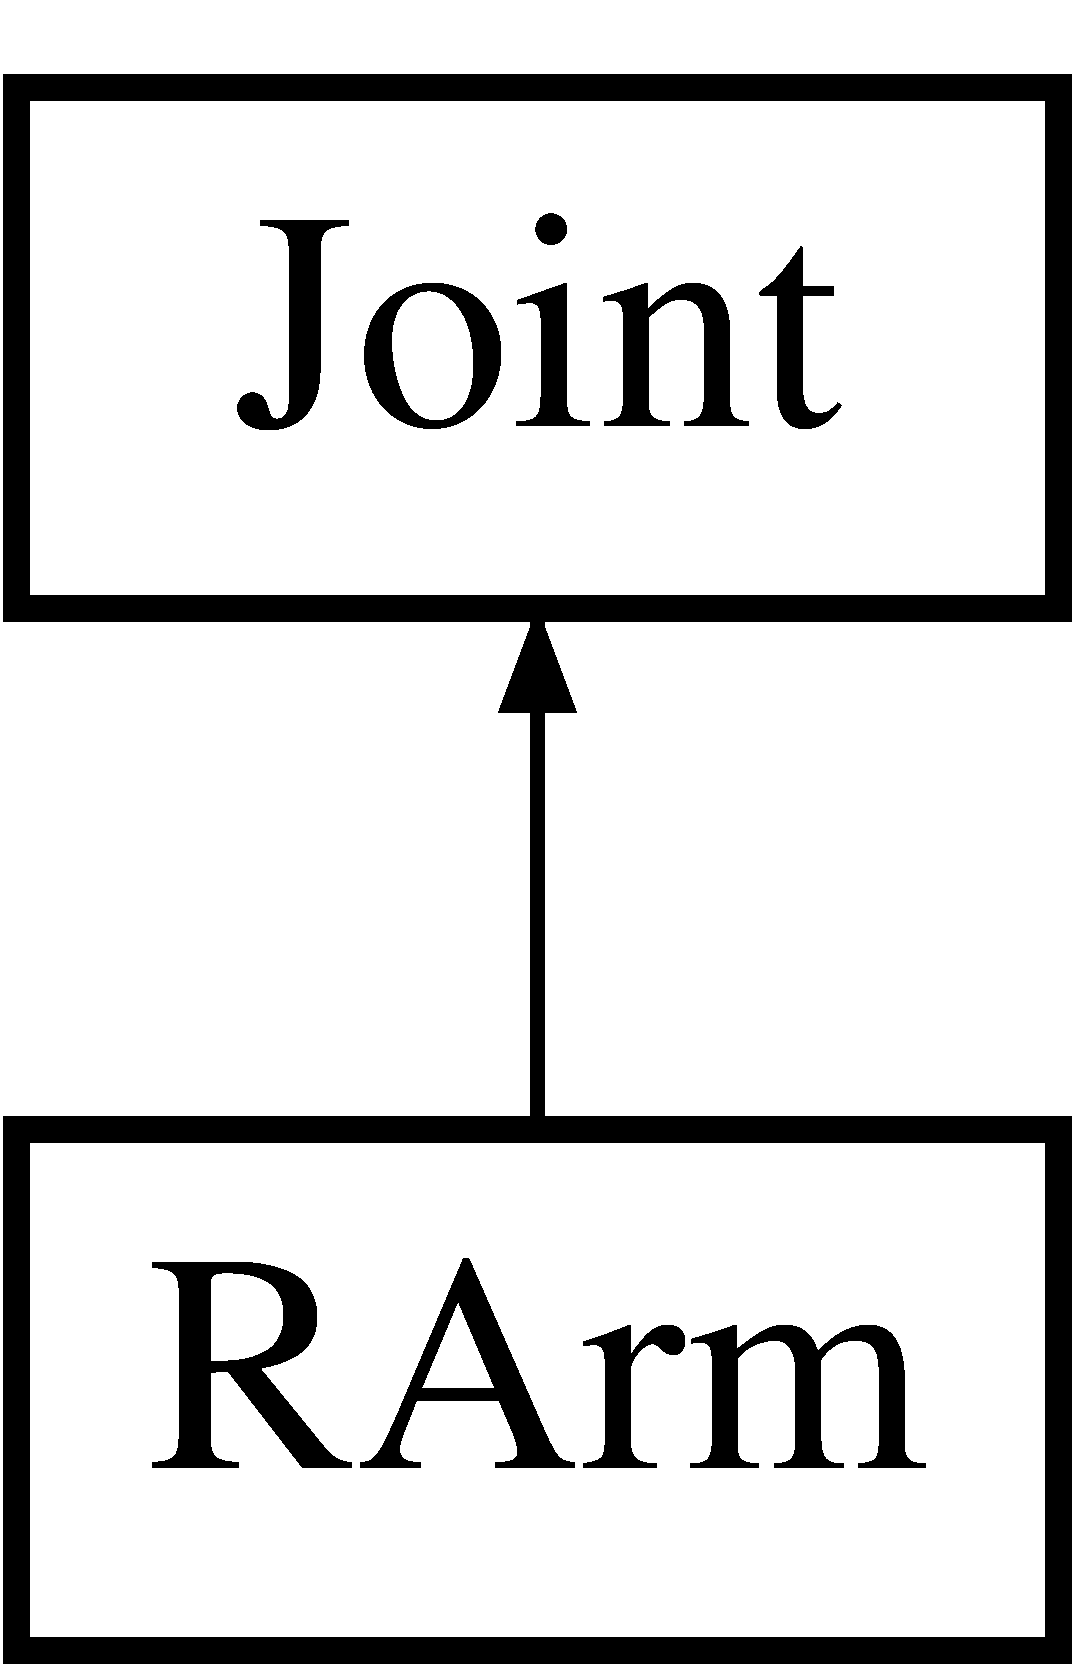
\includegraphics[height=2.000000cm]{class_r_arm}
\end{center}
\end{figure}
\subsection*{\-Public \-Member \-Functions}
\begin{itemize}
\item 
virtual float \hyperlink{class_r_arm_a5c91fecc7fea6e246ce87aac487bde4f}{get\-Elbow\-Roll} (\-Xn\-User\-I\-D, xn\-::\-User\-Generator)
\begin{itemize}\small\item\em \-Obtiene el ángulo que se determina a partir del kinect del codo. \end{itemize}\item 
\hypertarget{class_r_arm_a4788e34770371ab502e1a0d35ec41231}{virtual float \hyperlink{class_r_arm_a4788e34770371ab502e1a0d35ec41231}{set\-Elbow\-Roll} (float, float \&, float \&)}\label{class_r_arm_a4788e34770371ab502e1a0d35ec41231}

\begin{itemize}\small\item\em \-Genera el ángulo al que se necesita mover el \-N\-A\-O. \end{itemize}\item 
\hypertarget{class_r_arm_a273b56a909d68b769dc1ee4aab39fa55}{virtual float \hyperlink{class_r_arm_a273b56a909d68b769dc1ee4aab39fa55}{get\-Shoulder\-Roll} (\-Xn\-User\-I\-D, xn\-::\-User\-Generator)}\label{class_r_arm_a273b56a909d68b769dc1ee4aab39fa55}

\begin{itemize}\small\item\em \-Obtiene el ángulo que se determina a partir del kinect del hombro. \end{itemize}\item 
\hypertarget{class_r_arm_aef1de77829d8fe536eed27639408771b}{virtual float \hyperlink{class_r_arm_aef1de77829d8fe536eed27639408771b}{set\-Shoulder\-Roll} (float, float \&, float \&)}\label{class_r_arm_aef1de77829d8fe536eed27639408771b}

\begin{itemize}\small\item\em \-Genera el ángulo necesario al que se debe mover el \-N\-A\-O. \end{itemize}\item
\hypertarget{class_r_arm_a2647e80238d7767765777fae35ec92bb}{virtual float \hyperlink{class_r_arm_a2647e80238d7767765777fae35ec92bb}{get\-Elbow\-Yaw} (\-Xn\-User\-I\-D, xn\-::\-User\-Generator)}\label{class_r_arm_a2647e80238d7767765777fae35ec92bb}

\item 
\hypertarget{class_r_arm_a72b8946ae53bc1697bdd8371468334ba}{virtual float \hyperlink{class_r_arm_a72b8946ae53bc1697bdd8371468334ba}{set\-Elbow\-Yaw} (float, float \&, float \&)}\label{class_r_arm_a72b8946ae53bc1697bdd8371468334ba}

\end{itemize}

\subsection{\-Descripción \-Detallada}
\-Aquí se describe la clase derivada \char`\"{}\-RArm\char`\"{}. 

\subsection{\-Documentación de \-Función \-Miembro}
\hypertarget{class_r_arm_a5c91fecc7fea6e246ce87aac487bde4f}{\index{\-R\-Arm@{\-R\-Arm}!get\-Elbow\-Roll@{get\-Elbow\-Roll}}
\index{get\-Elbow\-Roll@{get\-Elbow\-Roll}!RArm@{\-R\-Arm}}
\subsubsection[{get\-Elbow\-Roll}]{\setlength{\rightskip}{0pt plus 5cm}float {\bf \-R\-Arm\-::get\-Elbow\-Roll} (
[{\-Xn\-User\-I\-D}]{user, }
[{xn\-::\-User\-Generator}]{guser}
)\hspace{0.3cm}{\ttfamily  \mbox{[}virtual\mbox{]}}}}\label{class_r_arm_a5c91fecc7fea6e246ce87aac487bde4f}


\-Primero se obtienen los puntos que van a determinar el ángulo de codo, se toman los puntos de la muñeca, codo y hombro.\\
\-Luego, utilizando las funciones descritas en la función base Joint, se procede a determinar el ángulo para el movimiento del codo. 

\-La documentación para esta clase fue generada apartir de los archivos\-:\begin{itemize}
\item 
joint.\-h\item 
rarm.\-cpp\end{itemize}

\hypertarget{class_r_leg}{\section{R\-Leg Class Reference}
\label{class_r_leg}\index{R\-Leg@{R\-Leg}}
}
Inheritance diagram for R\-Leg\-:\begin{figure}[H]
\begin{center}
\leavevmode
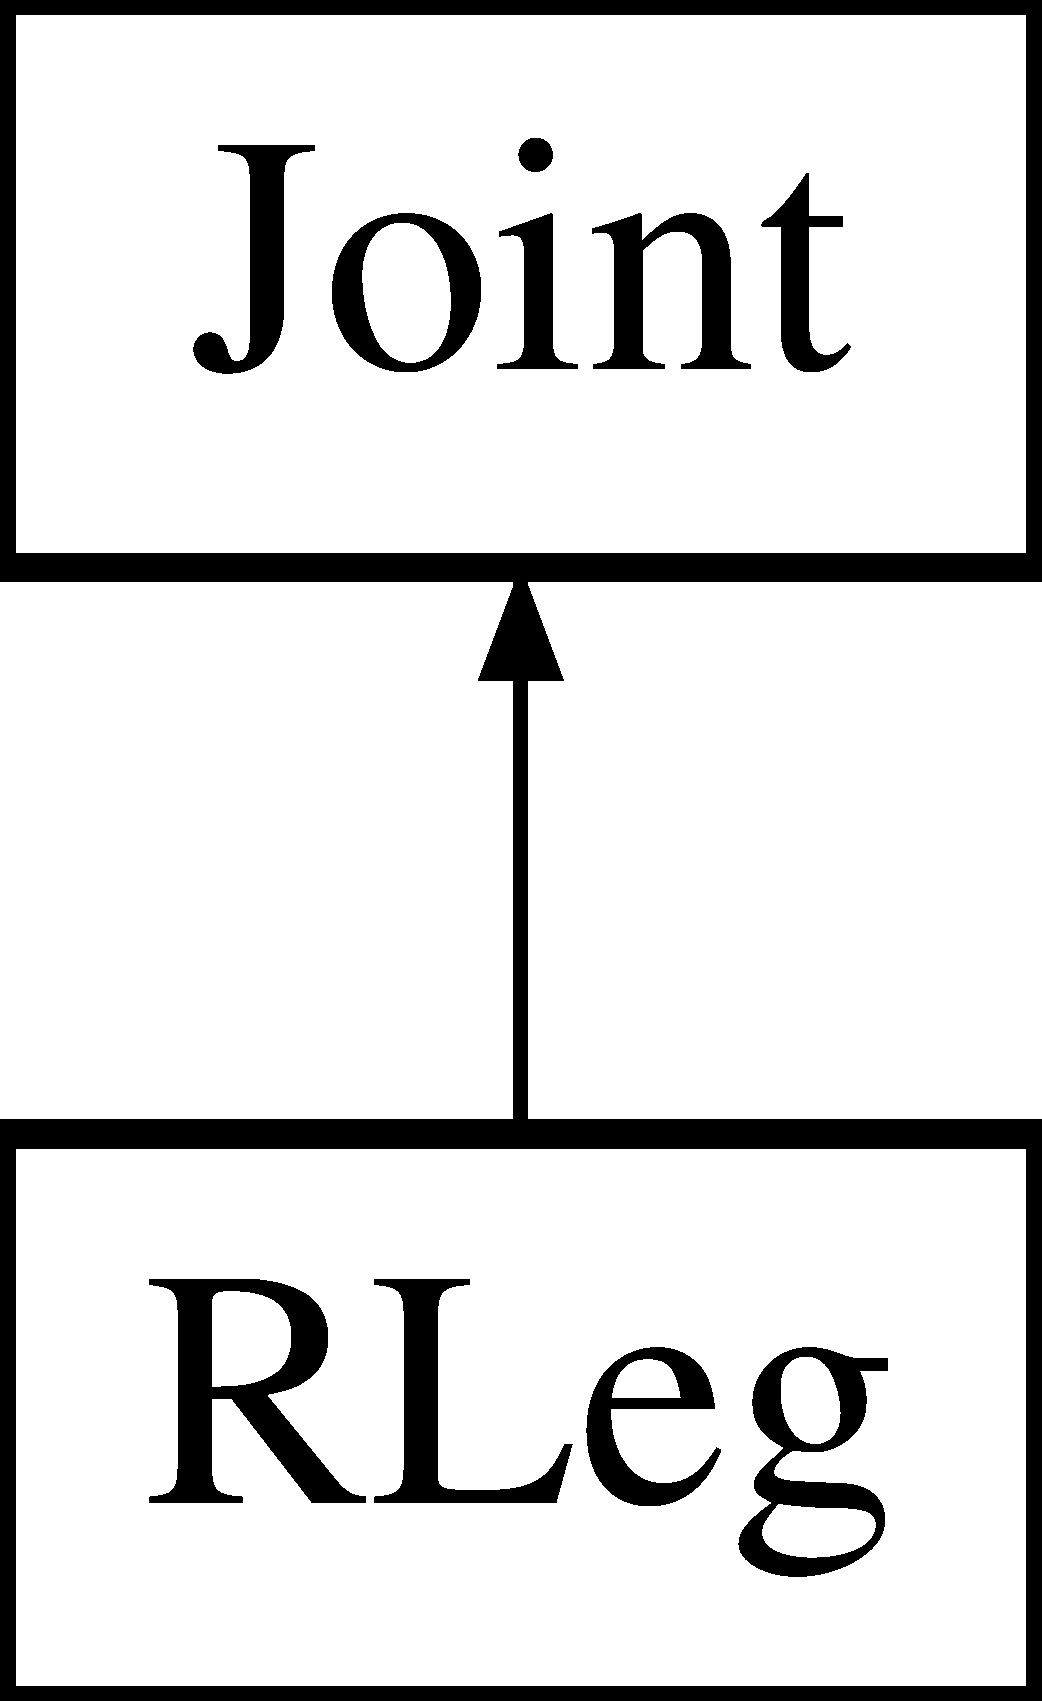
\includegraphics[height=2.000000cm]{class_r_leg}
\end{center}
\end{figure}
\subsection*{Public Member Functions}
\begin{DoxyCompactItemize}
\item 
virtual float \hyperlink{class_r_leg_a983e8da29c577737694dc72a9573fc5c}{get\-Hip\-Roll} (Xn\-User\-I\-D, xn\-::\-User\-Generator)
\begin{DoxyCompactList}\small\item\em Obtiene el angulo que se determina a partir del kinect del hombro. \end{DoxyCompactList}\item 
\hypertarget{class_r_leg_a44386f31cf1afb03ab3f433a0189d820}{virtual float \hyperlink{class_r_leg_a44386f31cf1afb03ab3f433a0189d820}{set\-Hip\-Roll} (float, float \&, float \&)}\label{class_r_leg_a44386f31cf1afb03ab3f433a0189d820}

\begin{DoxyCompactList}\small\item\em Genera el angulo necesario para mover el N\-A\-O. \end{DoxyCompactList}\item 
\hypertarget{class_r_leg_a1e66a29fe07ec16275f86bffe7482fee}{virtual float \hyperlink{class_r_leg_a1e66a29fe07ec16275f86bffe7482fee}{get\-Knee\-Pitch} (Xn\-User\-I\-D, xn\-::\-User\-Generator)}\label{class_r_leg_a1e66a29fe07ec16275f86bffe7482fee}

\begin{DoxyCompactList}\small\item\em Obtiene el angulo que se determina a partir del kinect. \end{DoxyCompactList}\item 
\hypertarget{class_r_leg_a65c0d913ed2c07515cd178b190b4287c}{virtual float \hyperlink{class_r_leg_a65c0d913ed2c07515cd178b190b4287c}{set\-Knee\-Pitch} (float, float \&, float \&)}\label{class_r_leg_a65c0d913ed2c07515cd178b190b4287c}

\begin{DoxyCompactList}\small\item\em Genera el angulo necesario para mover el N\-A\-O. \end{DoxyCompactList}\item 
\hypertarget{class_r_leg_aa8a63cd3f3d06ace1566a531b5213860}{virtual float \hyperlink{class_r_leg_aa8a63cd3f3d06ace1566a531b5213860}{get\-Ankle\-Pitch} (Xn\-User\-I\-D, xn\-::\-User\-Generator)}\label{class_r_leg_aa8a63cd3f3d06ace1566a531b5213860}

\begin{DoxyCompactList}\small\item\em Obtiene el angulo que se determina a partir del kinect. \end{DoxyCompactList}\item 
\hypertarget{class_r_leg_a6ac413efc8dc05dce14096d9797f9149}{virtual float \hyperlink{class_r_leg_a6ac413efc8dc05dce14096d9797f9149}{set\-Ankle\-Pitch} (float, float \&, float \&)}\label{class_r_leg_a6ac413efc8dc05dce14096d9797f9149}

\begin{DoxyCompactList}\small\item\em Genera angulo para mover N\-A\-O. \end{DoxyCompactList}\end{DoxyCompactItemize}


\subsection{Member Function Documentation}
\hypertarget{class_r_leg_a983e8da29c577737694dc72a9573fc5c}{\index{R\-Leg@{R\-Leg}!get\-Hip\-Roll@{get\-Hip\-Roll}}
\index{get\-Hip\-Roll@{get\-Hip\-Roll}!RLeg@{R\-Leg}}
\subsubsection[{get\-Hip\-Roll}]{\setlength{\rightskip}{0pt plus 5cm}float R\-Leg\-::get\-Hip\-Roll (
\begin{DoxyParamCaption}
\item[{Xn\-User\-I\-D}]{user, }
\item[{xn\-::\-User\-Generator}]{guser}
\end{DoxyParamCaption}
)\hspace{0.3cm}{\ttfamily [virtual]}}}\label{class_r_leg_a983e8da29c577737694dc72a9573fc5c}


Obtiene el angulo que se determina a partir del kinect del hombro. 

Obtiene el angulo real dado por el kinect del movimiento del codo. 

The documentation for this class was generated from the following files\-:\begin{DoxyCompactItemize}
\item 
/home/daniel/\-U\-C\-R/\-Ey\-A\-Team/kinect/\-Open\-N\-I\-\_\-\-N\-I\-T\-E\-\_\-\-Installer-\/\-Linux64-\/0.\-27/\-Open\-N\-I-\/\-Bin-\/\-Dev-\/\-Linux-\/x64-\/v1.\-5.\-4.\-0/\-Samples/\-Ni\-Simple\-Skeleton/kinao/joint.\-h\item 
/home/daniel/\-U\-C\-R/\-Ey\-A\-Team/kinect/\-Open\-N\-I\-\_\-\-N\-I\-T\-E\-\_\-\-Installer-\/\-Linux64-\/0.\-27/\-Open\-N\-I-\/\-Bin-\/\-Dev-\/\-Linux-\/x64-\/v1.\-5.\-4.\-0/\-Samples/\-Ni\-Simple\-Skeleton/kinao/rleg.\-cpp\end{DoxyCompactItemize}

\hypertarget{struct_xn_reference_axis}{\section{Xn\-Reference\-Axis Struct Reference}
\label{struct_xn_reference_axis}\index{Xn\-Reference\-Axis@{Xn\-Reference\-Axis}}
}


Definimos un struct \hyperlink{struct_xn_reference_axis}{Xn\-Reference\-Axis} para construir ejes de referencia a partir de vectores.  


\subsection*{Public Attributes}
\begin{DoxyCompactItemize}
\item 
\hypertarget{struct_xn_reference_axis_a4ac206c12a05a55ca3b556525f53c072}{Xn\-Vector3\-D {\bfseries New\-X}}\label{struct_xn_reference_axis_a4ac206c12a05a55ca3b556525f53c072}

\item 
\hypertarget{struct_xn_reference_axis_abe619023a45ec8a7c827f9e42aedf070}{Xn\-Vector3\-D \hyperlink{struct_xn_reference_axis_abe619023a45ec8a7c827f9e42aedf070}{New\-Y}}\label{struct_xn_reference_axis_abe619023a45ec8a7c827f9e42aedf070}

\begin{DoxyCompactList}\small\item\em Es un vector de coordenadas del nuevo eje en X. \end{DoxyCompactList}\item 
\hypertarget{struct_xn_reference_axis_a149a25a6e03ea545d2e99b03a825da51}{Xn\-Vector3\-D \hyperlink{struct_xn_reference_axis_a149a25a6e03ea545d2e99b03a825da51}{New\-Z}}\label{struct_xn_reference_axis_a149a25a6e03ea545d2e99b03a825da51}

\begin{DoxyCompactList}\small\item\em Es un vector de coordenadas del nuevo eje en Y. \end{DoxyCompactList}\end{DoxyCompactItemize}


\subsection{Detailed Description}
Definimos un struct \hyperlink{struct_xn_reference_axis}{Xn\-Reference\-Axis} para construir ejes de referencia a partir de vectores. 

The documentation for this struct was generated from the following files\-:\begin{DoxyCompactItemize}
\item 
/home/daniel/\-U\-C\-R/\-Ey\-A\-Team/kinect/\-Open\-N\-I\-\_\-\-N\-I\-T\-E\-\_\-\-Installer-\/\-Linux64-\/0.\-27/\-Open\-N\-I-\/\-Bin-\/\-Dev-\/\-Linux-\/x64-\/v1.\-5.\-4.\-0/\-Samples/\-Ni\-Simple\-Skeleton/kinao/definition.\-h\item 
/home/daniel/\-U\-C\-R/\-Ey\-A\-Team/kinect/\-Open\-N\-I\-\_\-\-N\-I\-T\-E\-\_\-\-Installer-\/\-Linux64-\/0.\-27/\-Open\-N\-I-\/\-Bin-\/\-Dev-\/\-Linux-\/x64-\/v1.\-5.\-4.\-0/\-Samples/\-Ni\-Simple\-Skeleton/kinao/normal.\-cpp\end{DoxyCompactItemize}

%--- End generated contents ---

% Index
\newpage
\phantomsection
\addcontentsline{toc}{chapter}{Index}
\printindex

\end{document}
